\documentclass{frontiersSCNS}

\usepackage{url,lineno}
\usepackage{placeins}

\linenumbers

\copyrightyear{}
\pubyear{}

\def\journal{Bioinformatics and Computational Biology}
\def\DOI{}
\def\articleType{Methods Article}
\def\keyFont{\fontsize{8}{11}\helveticabold }
\def\firstAuthorLast{Chapman {et~al.}}
\def\Authors{Brad Chapman\,$^{1}$, Rory Kirchner\,$^{1}$ Oliver Hofmann\,$^{1}$ and Winston Hide\,$^{1,*}$}
\def\Address{$^{1}$Bioinformatics Core, Harvard School of Public Health, Department of Biostatistics, Boston, MA USA}
\def\corrAuthor{Winston Hide}
\def\corrAddress{Harvard School of Public Health, 655 Huntington Avenue Building II, Room 415 Boston, Massachusetts 02115 USA}
\def\corrEmail{whide @hsph.harvard.edu}

\begin{document}
\onecolumn
\firstpage{1}

\title[Community variant pipelines]{Community development of validated variant calling pipelines}
\author[\firstAuthorLast ]{\Authors}
\address{}
\correspondance{}
\extraAuth{}
\topic{Bioinformatics and genetic variation exploration}

\maketitle

\begin{abstract}

Exploratory and translational research relies on accurate
identification of genomic variants from populations, families
and cancer tumor/normal pairings. However, rapidly changing best
practice approaches in alignment and variant calling, coupled with
large data sizes, make it a challenge to develop scalable, accurate
pipelines that can remain up to date. Coordinated community development overcomes these
challenges by sharing testing and updates across groups relying on the
same infrastructure.

bcbio-nextgen is a distributed multi-architecture pipeline that
automates variant calling, validation and organization of results for
query and analysis. It creates an easily installable and widely
runnable infrastructure from best-practice tools, coupled with an
integrated methodology for assessing variant quality. We use the
bcbio-nextgen framework to provide comparisons of variant calling
methods and pipelines and identify key bottlenecks for scaling to large
collections of whole genome sequencing data.

The open-source, community-developed framework is freely available
from \url{https://github.com/chapmanb/bcbio-nextgen}.

\tiny
 \keyFont{ \section{Keywords:} Next Generation Sequencing, Variant detection,
   Quality control and validation, Community development, Open source software}
\end{abstract}

\section*{Introduction}

bcbio-nextgen provides a variant calling pipeline to accurately detect single
nucleotide polymorphisms (SNPs) and insertions/deletions (indels) from high
throughput sequencing data. It utilizes multiple best practice approaches for
alignment, alignment post-processing and variant calling, provides an integrated
mechanism to assess variant quality and interfaces with downstream tools for
variant analysis. Practically, it installs with a single command on multiple
computing architectures, scales to large whole genome analyses, and is community
developed. The goal is to provide a robust platform for moving from raw sequencing data
to high-quality variant calls that evolves as algorithms and sequencing
technologies change.

The pipeline utilizes existing algorithms, wrapping them in an easy to use and
scalable way. It provides software programming interfaces to enable new tools
and currently builds on a large number of reusable software packages:

\begin{itemize}
  \item Alignment: bwa~\citep{li_fast_2010}, bwa-mem~\citep{li_aligning_2013} and
    novoalign~\citep{novoalign}
  \item BAM alignment processing: samtools~\citep{li_sequence_2009},
    bamtools~\citep{bamtools}, Picard~\citep{picard},
    sambamba~\citep{sambamba} and pysam~\citep{pysam}
  \item Interval manipulation: BedTools~\citep{quinlan_bedtools:_2010} and
    pybedtools~\citep{dale_pybedtools:_2011}
  \item Variant calling: GATK~\citep{depristo_framework_2011} and
    FreeBayes~\citep{garrison_haplotype-based_2012}
\end{itemize}

The pipeline reports variant calling results both in standard VCF format and
as a ready to query database, making results analyzable by both
bioinformaticians and biologists familiar with SQL and command line tools.
snpEff~\citep{cingolani_program_2012} predicts effects associated with
identified variation and GEMINI provides the SQLite database associating
variants with a wide variety of genome annotations~\citep{paila_gemini:_2013}.

Three major components of bcbio-nextgen differentiate it from
both existing tools like HugeSeq \citep{lam_detecting_2012} and customized
in-house scripts:

\begin{itemize}
\item Quantifiable: It validates variant calls against known reference materials
  developed by the Genome in a Bottle consortium \citep{zook_integrating_2013}.
  Automating scoring and assessment of calls allows identification of
  improvements or regressions in variant identification as calling pipelines
  evolve. Incorporation of multiple variant calling approaches from Broad's GATK
  best practices \citep{van_der_auwera_fastq_2002} and the Marth lab's FreeBayes
  caller \citep{garrison_haplotype-based_2012} enables informed comparisons
  between algorithms.

\item Scalable: bcbio-nextgen handles large population studies with
  hundreds of whole genome samples by parallelizing on a wide variety
  of schedulers (LSF, SGE, Torque, SLURM) and multicore machines.

\item Community developed: Due to the focus on solving the problems
  of setting up and maintaining a complex analysis pipeline, multiple
  sequencing centers and research laboratories use bcbio-nextgen <<<SUCH AS
  AND REFER TO A TABLE OF THE SITES AT WHICH IT IS EMPLOYED TOGETEHR WITH THE ARCHITECTURES>>>>. We
  actively encourage contributors to the code base and make it easy to
  get started with a fully automated installer and updater that
  prepares all third party software and reference genomes.
\end{itemize}

\section*{Validation}

Alignment and variant calling algorithms are both diverse and rapidly
changing. Tools quickly become outdated and new approaches provide improved
resolution and speed. This continuous change requires flexible pipelines that
can incorporate new methods and iterate rapidly in response to updated tools. It
also requires integrated methods for ensuring that variant calling accuracy
improves with new changes, and for evaluating new methodologies against
established best practice.

bcbio-nextgen includes an automated approach to validate calling methods against
known reference materials. A high quality NA12878 reference genome developed by
the Genome in a Bottle consortium \citep{zook_integrating_2013} provides a
baseline dataset for comparison. The evaluation dataset is a NA12878 clinical
exome contributed by EdgeBio. The process of retrieving the data and running the
evaluation is fully documented
(\url{https://bcbio-nextgen.readthedocs.org/en/latest/contents/testing.html#exome-with-validation-against-reference-materials}).

As an example of the usefulness of having this integrated validation system, we
evaluated three different current variant callers:

\begin{itemize}
\item FreeBayes (v0.9.9.2-18): A haplotype-based Bayesian caller, filtering
  calls with a hard filter based on depth and quality (DP < 5; QUAL < 20).

\item GATK UnifiedGenotyper (2.7-2): GATK’s Bayesian caller, with
  calls filtered using GATK's recommended hard filters.

\item GATK HaplotypeCaller (2.7-2): A GATK variant caller which local haplotype
  re-assembly around variant regions. We also filtered these calls using
  recommended hard filters.
\end{itemize}

Following alignment with bwa-mem (0.7.5a), we additionally post-processed
the BAM files with two methods:

\begin{itemize}
\item GATK’s best practices (2.7-2): This involves de-duplication with Picard
  MarkDuplicates, GATK base quality score recalibration and GATK realignment
  around indels.
\item Minimal post-processing: with de-duplication using samtools rmdup and no
  realignment or recalibration.
\end{itemize}

\FloatBarrier

Figures~\ref{fig:01} and \ref{fig:02} show comparisons to the Genome in a Bottle
reference materials for the GATK best practice and minimal BAM preference
methods, respectively.

\begin{figure}[tbp]
\begin{center}
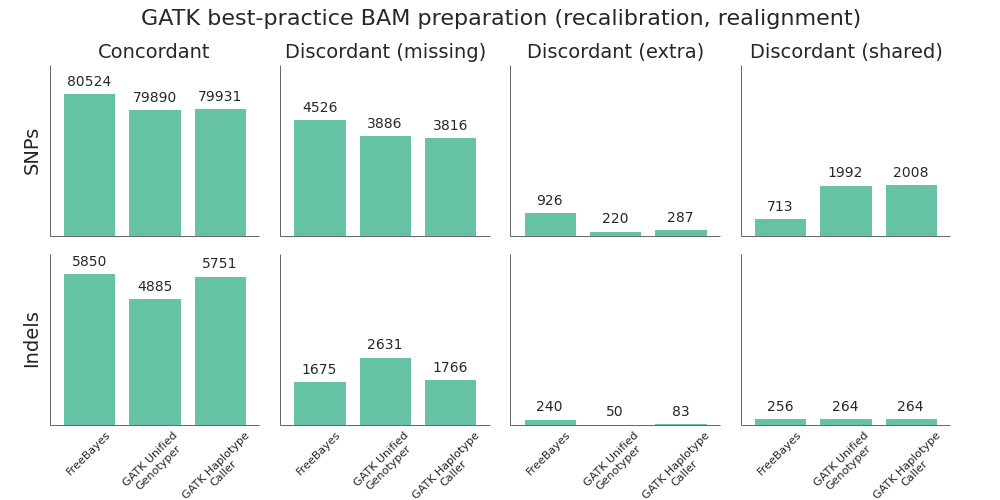
\includegraphics[width=0.9\textwidth]{validation-gatkprep}
\end{center}
 \textbf{\refstepcounter{figure}\label{fig:01} Figure \arabic{figure}.}{
   Validation results for three variant calling methods using GATK best practice
 post-alignment preparation (de-duplication, realignment around indels and base
 quality recalibration). Realigning variant callers (GATK HaplotypeCaller and
 FreeBayes) have equal sensitivity and specificity in calling SNPs but provide
 improved resolution of indels. FreeBayes performs on par with GATK
 HaplotypeCaller methods. Discordant variants are in 3 categories. Missing: not
 present in evaluation but present in reference (potential false negatives),
 Extra: present in evaluation but not in reference (potential false
 positives). Shared: present in both but different due to
 heterozygote/homozygote call or alleles called.}
\end{figure}

\begin{figure}[tbp]
\begin{center}
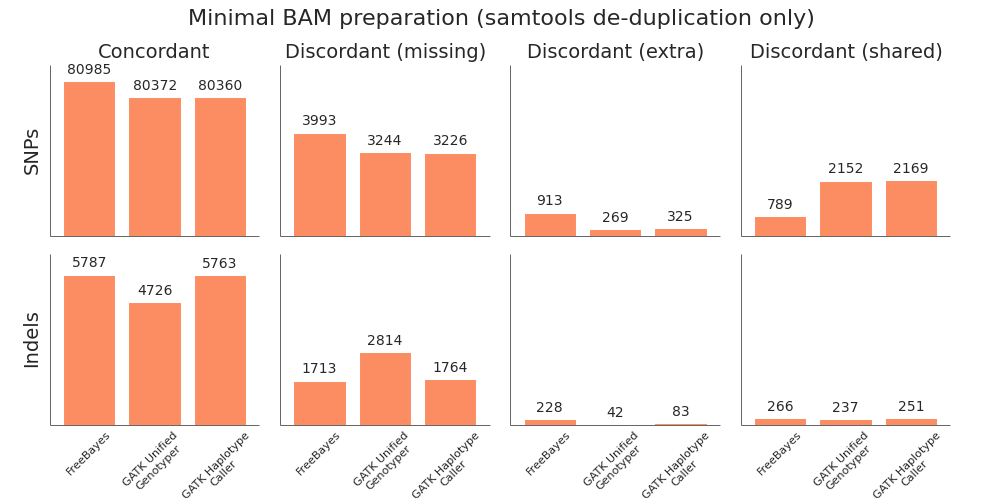
\includegraphics[width=0.9\textwidth]{validation-noprep}
\end{center}
 \textbf{\refstepcounter{figure}\label{fig:02} Figure \arabic{figure}.}{
   Validation results for three variant calling methods using minimal BAM
   post-alignment preparation methods (only de-duplication). Results are
   equivalent to those seen using the more time intensive GATK best practice
   approach when using realigning variant callers (GATK HaplotypeCaller and FreeBayes).}
\end{figure}

The comparison identified three areas to consider for future variant calling.
First, FreeBayes outperforms the GATK callers on both SNP and indel calling. The
most recent versions of FreeBayes have improved sensitivity and specificity
which puts them on par with GATK HaplotypeCaller. Second, GATK HaplotypeCaller
is all around better than the UnifiedGenotyper. In previous GATK versions,
UnifiedGenotyper performed better on SNPs and HaplotypeCaller
better on indels, but the recent improvements in GATK 2.7 have resolved the
difference in SNP calling. Finally, skipping base recalibration and indel
realignment had almost no impact on the quality of resulting variant calls when
using a realigning caller.  While GATK UnifiedGenotyper suffers during indel
calling without recalibration and realignment, both HaplotypeCaller and
FreeBayes perform as good or better without these steps.

The main benefit of validation is to enable experiments that quantitatively
assess widely held approaches. We expect best practices to change with new
releases and algorithms. The automated assessment mechanism allows
bcbio-nextgen to track and adapt to continuously improving tools.

\FloatBarrier

\section*{Scaling}

The second differentiating feature of bcbio-nextgen is the ability to scale to
handle large population whole genome datasets on a wide variety of
architectures. The pipeline runs in parallel on single multicore machines or on
clusters with a shared filesystem and scheduler. It utilizes the general purpose
IPython parallel infrastructure \citep{IPython}, which supports multiple
schedulers including LSF, SGE, SLURM, and Torque. This infrastructure allows
jobs to adapt to increased scale or system changes without adjusting the
underlying configuration or code.

To utilize large cluster architectures, bcbio-nextgen parallelizes
processing at multiple steps:

\begin{itemize}
  \item Alignment -- Block gzipping (bgzip) and indexing of sequencing reads with
    grabix~\citep{grabix} allows alignment processing in blocks. The split size
    for each alignment is configurable to match available processing cores.
  \item Alignment post-processing -- Following alignment the pipeline assesses
    callable regions in each sample, identifying regions with no coverage to use
    as analysis breakpoints. Each chromosomal region between regions of no coverage
    provides an independent section for parallel processing (Figure~\ref{fig:03}).
  \item Variant calling -- Variant processing parallelizes using the same
    chromosomal blocks identified during alignment post-processing. For
    population and family based calling, variant calls occur simultaneously for
    all batched samples in a region.
  \item Identification of callable regions, BAM merging and indexing, quality
    control, and GEMINI database preparation -- All of these steps allow shared
    memory parallel processing, which the pipeline enables by launching cluster
    jobs with multiple cores on a single machine.
\end{itemize}

\begin{figure}[tbp]
\begin{center}
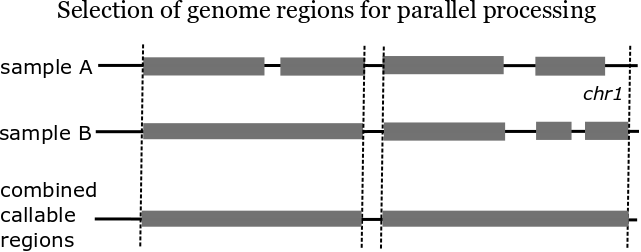
\includegraphics[width=0.5\textwidth]{parallel-genome}
\end{center}
 \textbf{\refstepcounter{figure}\label{fig:03} Figure \arabic{figure}.}{
   Identification of shared no coverage regions between multiple samples. Each
   no coverage region breaks the genome into chunks allowing parallel processing.}
\end{figure}

Within each independently running parallel process, bcbio-nextgen controls
memory usage and disk IO to maximize the throughput of multiple simultaneous
processes.  An input configuration files specifies available memory usage for
programs that allow memory restrictions, and expected memory usage for those
that do not. These inputs allow for an accurate estimate of memory consumption and
bcbio-nextgen avoids overscheduling jobs relative to available memory on each
machine. Similarly, simultaneous disk IO on shared filesystems is a common
bottleneck during processing. bcbio-nextgen minimizes this by use of streaming
piped processing steps where supported by the underlying tools. As an example,
the alignment steps converts output into standard sorted BAM files via use of
unix pipes, avoiding writing intermediates to disk.

These scaling approaches enable simultaneous processing of large whole genome
population samples. As an example, Table\ref{Tab:01} shows timing results from
running 60 whole genome Illumina samples with 30x coverage through a full
alignment, variant calling, analysis and quality control pipeline. The example
uses Dell's Active Infrastructure~\citep{dell} with 400 cores, 3Gb of memory per
core and a Lustre filesystem connected on an Infiniband network.  Processing 60
samples in 5 days is an efffective time of 2 hours/sample when processing large
families. Single whole genome samples typically process in less than a day with
100 cores.

\begin{table}[!t]
\processtable{Processing times for 60 whole genome Illumina samples (30x) on 400 cores\label{Tab:01}}
{\begin{tabular}{lll}\toprule
Step & Time & Processes \\
\midrule
Alignment preparation & 13 hours & BAM to fastq; bgzip; grabix index \\
Alignment & 30 hours & bwa-mem alignment in parts \\
BAM merge & 7 hours & Merge alignment parts \\
Alignment post-processing & 6 hours & Calculate callable regions \\
Post-alignment BAM preparation & 6 hours & De-duplication \\
Variant calling & 23 hours & FreeBayes \\
Variant post-processing & 2 hours & Combine variant files; annotate with GATK and snpEff \\
BAM merging & 6 hours & Combine post-processed BAM file sections \\
GEMINI & 3 hours & Create GEMINI SQLite database \\
Quality Control & 5 hours & FastQC, alignment and variant statistics \\
\midrule
Total & 5 days & \\
\botrule
\end{tabular}}{}
\end{table}

\FloatBarrier

\section*{Community development}

A final unique aspect of the pipeline is a strong focus on community development
and broad usability. We believe that good quality scalable variant calling is a
shared problem faced in multiple research laboratories, core facilities and
companies.  By pooling resources, a community developed framework overcomes the
inherent difficulties associated with maintaining and extending rapidly changing
pipelines.

To achieve wide usability, bcbio-nextgen installs on multiple unix-based operating
systems and cluster types. An automated installer built on
CloudBioLinux~\citep{krampis_cloud_2012} installs both the bcbio-nextgen Python
framework as well as all associated tools and pre-indexed genomic
data. Installation is fully documented
(\url{https://bcbio-nextgen.readthedocs.org/en/latest/contents/installation.html})
and uses the same automated process to provide updates for new versions of the
pipeline and tools. It includes a full test suite as well as example exome and
genome datasets for ensuring correct installation and scaling
(\url{https://bcbio-nextgen.readthedocs.org/en/latest/contents/testing.html}).

\section*{Future work}

By removing installation and infrastructure integration hurdles,
bcbio-nextgen has an active user community with regular contributions from
outside our core group. We continue to actively develop the framework to increase
the scope and currently active projects include:

\begin{itemize}
  \item Coverage -- Assessment of coverage in gene regions of interest, allowing
    identification of regions without effective coverage for calling.
  \item Structural variation -- Detection of large scale events (duplications,
    deletions and inversions) as well as identification of copy number variations.
  \item Cancer tumor/normal -- Integration and evaluation of cancer-specific
    paired callers.
  \item RNA-seq --  Identify differentially expressed transcripts and evaluate
    performance of aligners and transcript resolution methods.
  \item Cloud computing -- Enable native support for cloud providers such as
    Amazon, making the pipeline readily usable by researchers without local
    compute infrastructure.
  \item Reproducibility and provenance -- Provide versioned, locally isolated
    Linux containers using Docker to improve the ability to trace and re-run
    analyses.
  \item Accessibility -- Interface with web-based biologist targeted front ends
    such as Galaxy (\cite{goecks_galaxy:_2010};
    \cite{giardine_galaxy:_2005}; \cite{blankenberg_galaxy:_2010}).
\end{itemize}

In summary, bcbio-nextgen provides an automated pipeline to identify and
validate genomic variations in high throughput sequencing data. The
pipeline scales to handle large population studies by minimizing computational
bottlenecks and integrating with multiple cluster architectures. The pipeline is
open-source, documented and we welcome community contributions.

\section*{Acknowledgments}

Thanks to John Morrissey and James Cuff at Harvard Faculty of Arts and Science
Research Computing, and Glen Otero and William Cottay at Dell Life Sciences for
compute infrastructure and support. Thank you to the open-source community for
feedback, reports, code fixes and contributions: Miika Ahdesmaki, Luca Beltrame,
Guillermo Carrasco, Peter Cock, Mario Giovacchini, Jakub Nowacki, Brent
Pedersen, James Porter, Valentine Svensson, Paul Tang, Roman Valls, and Kevin
Ying. Justin Johnson and David Jenkins at EdgeBio contributed the NA12878
evaluation exome dataset.

\paragraph{Funding} Funding for variation evaluation provided by the Archon
Genomic X Prize foundation.

\bibliographystyle{frontiersinSCNS&ENG} % for Science and Engineering articles
\bibliography{chapman_bcbio}

\section*{Figures}

Figures go here after review.

\end{document}
